% mainfile: ../../../../master.tex
\subsection{Inventory of nucleic acid samples}
% The part of the label after the colon must match the file name. Otherwise,
% conditional compilation based on task labels does NOT work.
\label{task:20180315_cj0}
\tags{lab,smp,dna,rna}
\authors{cj}
%\files{}
%\persons{}

\begin{figure}[H] % position of the figure 
    \centering
    \caption{Picture of my nucleic acid samples in the storage box kept in freezer at -20\degree C}
    \label{fig:20180315_nucl_acid_samples_inventory}
    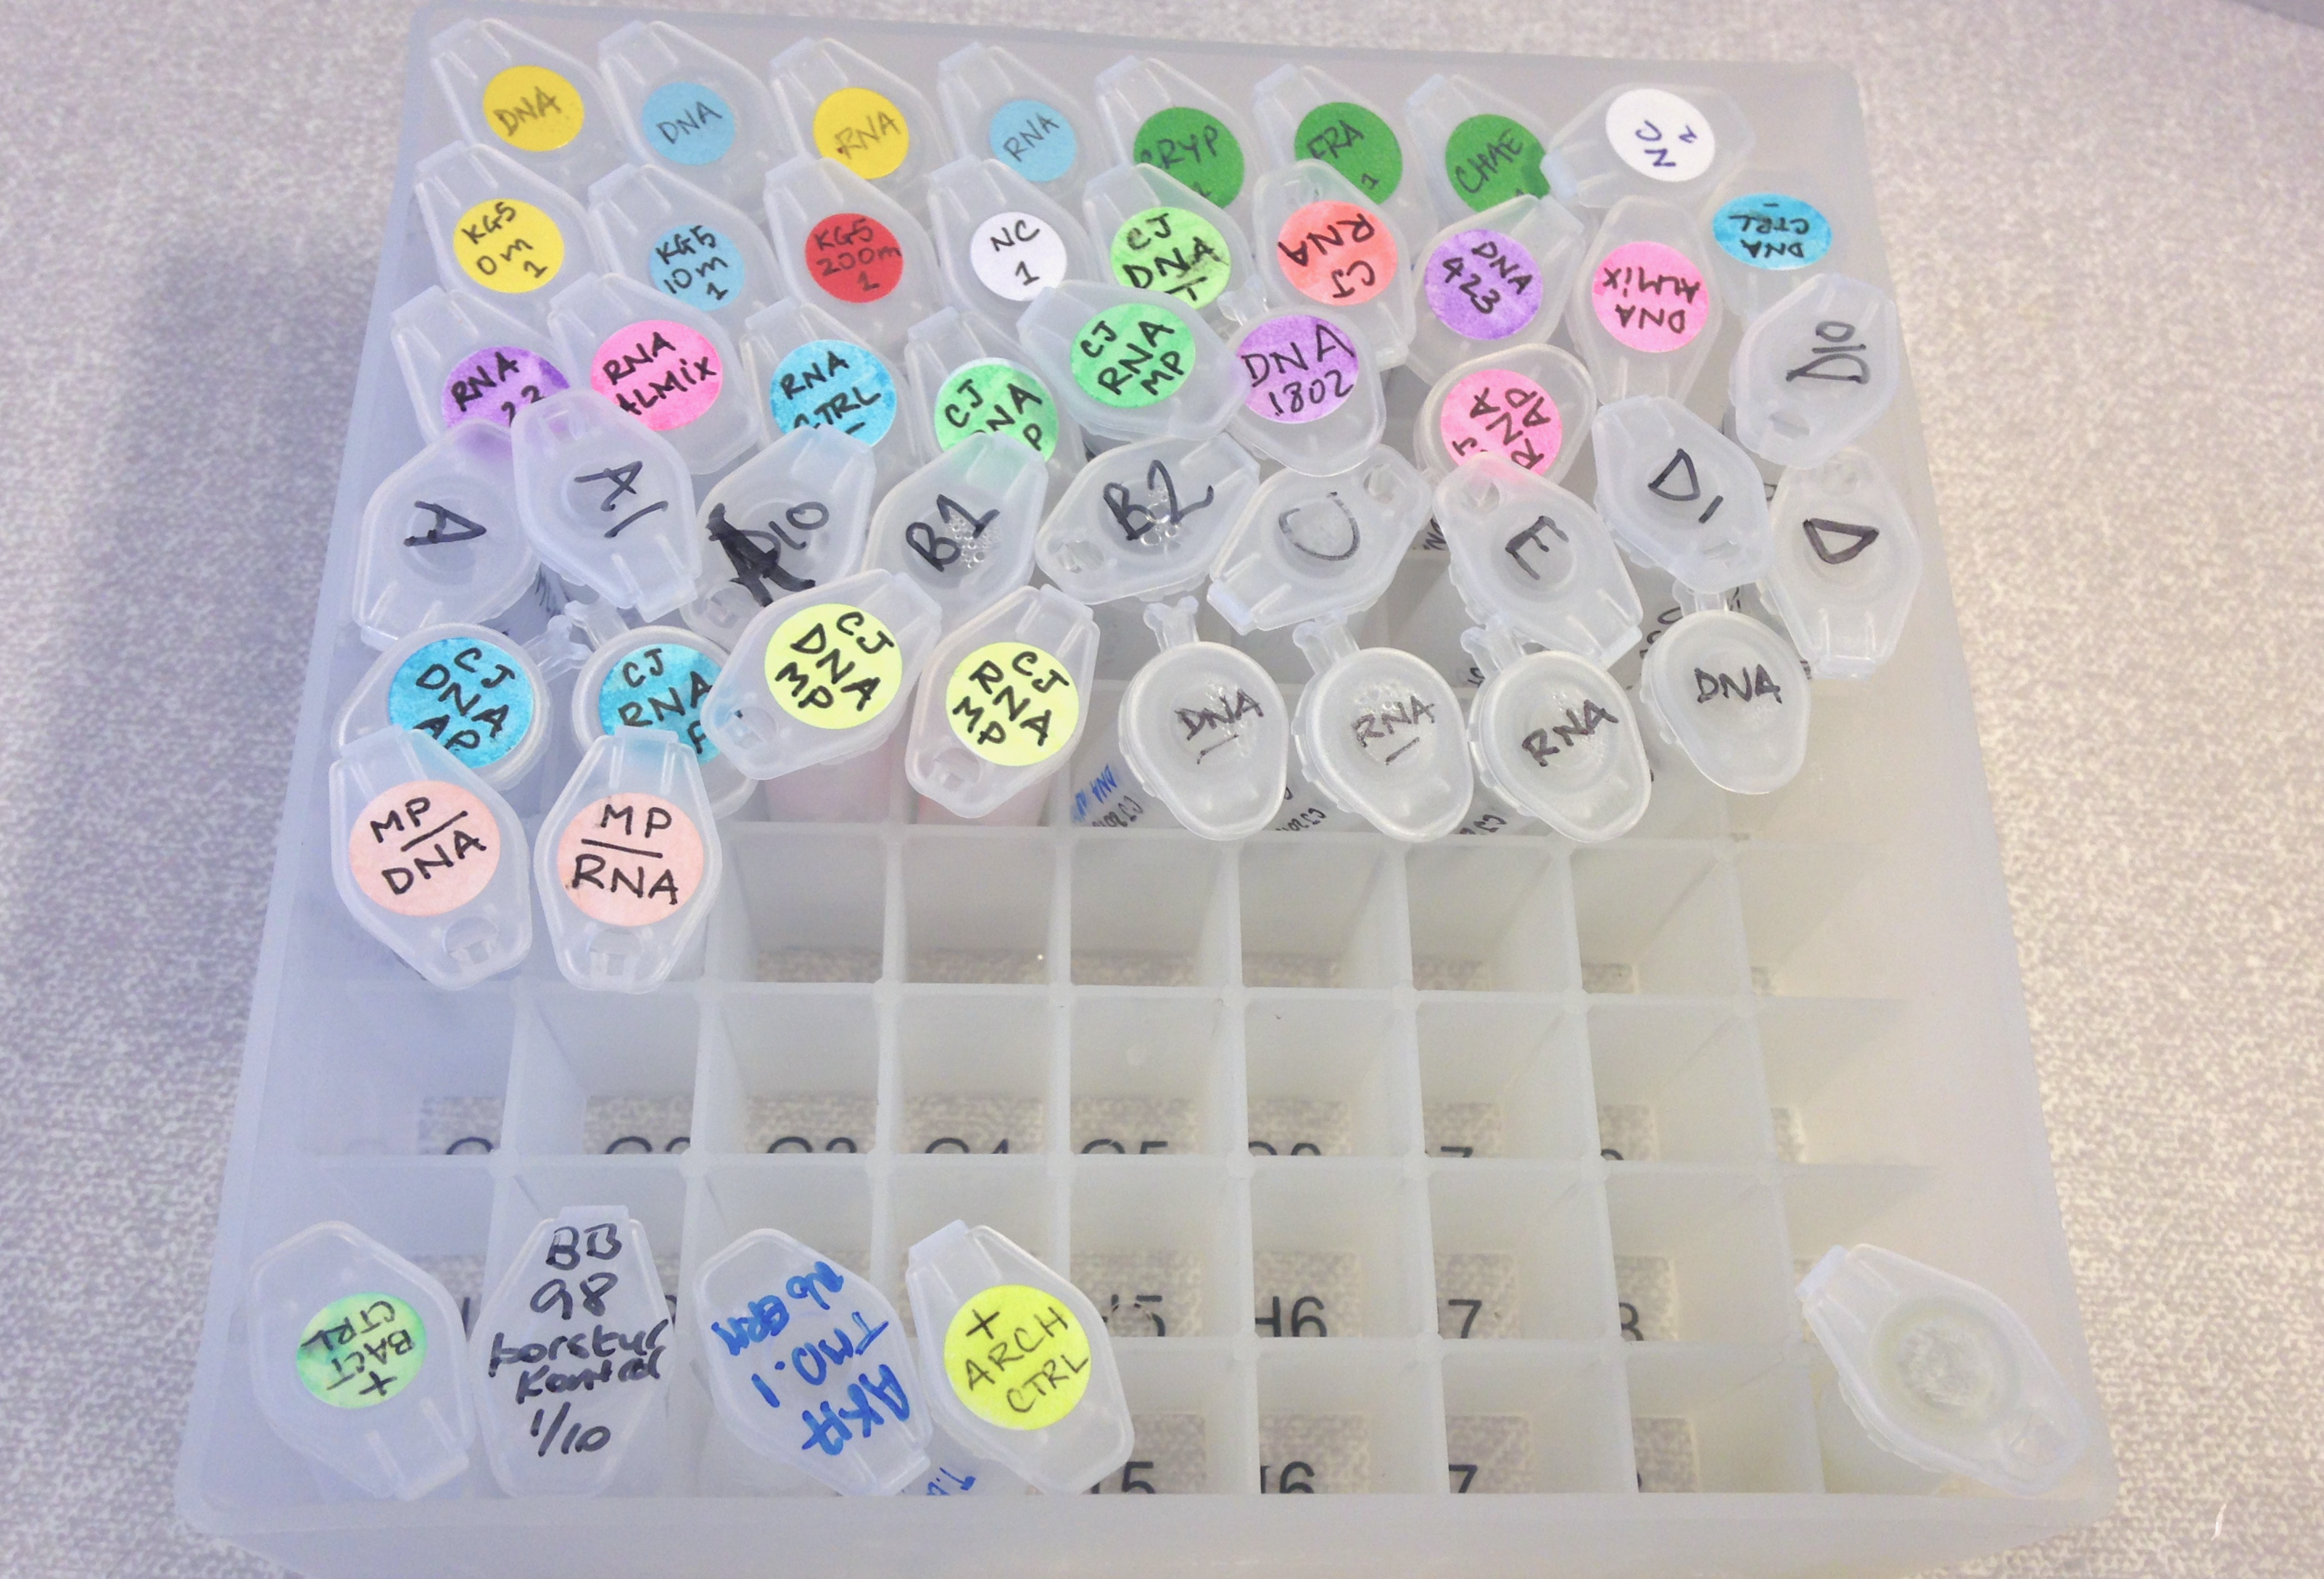
\includegraphics[width=\textwidth]{graphics/pic/20180315_nucl_acid_samples_inventory.png}
\end{figure}

\begin{table}[H]
\centering 
\resizebox{\textwidth}{!}{
\begin{tabular}{l l l l l r r}
\toprule
USER & LABEL & LABEL COLOR & BOX POSITION & EXTRACTION METHOD & STARTING MATERIAL & CONCENTRATION QUBIT \\
\midrule
\texttt{CJ} & DNA MP & GREEN & C4 & MasterPure & Micro-algae culture & 3,11 \\
\texttt{CJ} & RNA MP & GREEN & C5 & MasterPure & Micro-algae culture & 7,20 \\
\texttt{CJ} & DNA 1802 & PURPLE & C6 & AllPrep & Micro-algae culture & 2,44 \\
\texttt{CJ} & RNA AP & PINK & C7 & AllPrep & Micro-algae culture & 8,77 \\
\texttt{CJ} & DNA AP & BLUE & E1 & AllPrep & Micro-algae culture & 5,86 \\
\texttt{CJ} & RNA AP & BLUE & E2 & AllPrep & Micro-algae culture & 31,50 \\
\texttt{CJ} & DNA MP & YELLOW & E3 & MasterPure & Micro-algae culture & 18,20 \\
\texttt{CJ} & RNA MP & YELLOW & E4 & MasterPure & Micro-algae culture & 32,20 \\
\texttt{CJ} & DNA & NONE & E5 & AllPrep & Micro-algae culture & 7,71 \\
\texttt{CJ} & RNA & NONE & E6 & AllPrep & Micro-algae culture & 3,94 \\
\texttt{CJ} & DNA & NONE & E7 & AllPrep & Micro-algae culture & 3,45 \\
\texttt{CJ} & RNA & NONE & E8 & AllPrep & Micro-algae culture & 14,00 \\
\texttt{CJ} & MP DNA & PEACH & F1 & MasterPure & Micro-algae culture & 17,00 \\
\texttt{CJ} & MP RNA & PEACH & F2 & MasterPure & Micro-algae culture & 7,19 \\
\bottomrule
\end{tabular}
}
\end{table}
